\label{conclusions}
This section presents a summary of the results from previous chapters, lists
important branch prediction results and discoveries, compares our results with
LaMarca's and discusses important cache results, discusses the best sort that we
found in a number of catagories, and suggests contributions made to computer
science by this research.

\section{Results Summary}


\subsection{Elementary Sorts}

We found that insertion sort has the best performance of any of the elementary
sorts, with fewer instructions and cache misses than any other elementary sort,
and exactly one branch misprediction per key. Selection sort also has very few
branch mispredictions, and our results match figures created using Knuth's
harmonics formula. We found that bubblesort and shakersort have poor branch
prediction performance, and that this cripples their performance, especially
compared to selection sort which is otherwise similar in behaviour. We
determined that bubblesort has better branch performance at the start and end of
its sorting, than in the middle.

We also found that reducing the number of runs performed by shakersort and
bubblesort is counter-productive due to additional book-keeping cost. We found
that of the elementary sorts, only insertion sort has good cache performance, as
the others do not exploit any temporal locality.


\subsection{Heapsort}

The cache optimized heaps perform better than the non-optimized versions. At the
cost of a slightly increased instruction count, the number of cache misses can
be greatly reduced, and the overall performance of our 8-heap is significantly
better than the unoptimized version. This is despite our finding of that
increasing the fanout increases branch mispredictions.

Additionally, we created an improvement to heapsort using a 2-heap, which
removed the need for a sentinel, without introducing any more instructions. We
found that a $k$-ary heap has similar, though not the same, branch prediction
performance as selection sort, in that the fanout becomes more predictable the
larger it is.


\subsection{Mergesort}

We found that algorithm S has a lower instruction count than algorithm N, but
that this does not translate to better performance. Our results show also that
the level 1 cache needs to be taken into account, both in tiling and in
alignment; that the extra instructions in multi-mergesort make it slower than
tiled mergesort, and that multi-mergesort has regular access patterns during the
k-way merge, which can be taken advantage of by a two-level adaptive predictor.


\subsection{Quicksort}

Our results show base quicksort being the fastest of the quicksorts. We note our
lowest instruction count occurs with median-of-three partitioning. We also see
that using a binary search slows multi-quicksort down compared to a sequential
search due to branch mispredictions, but that both have too many extra
instructions to compete against memory-tuned quicksort. Despite being slower in
our tests, our simulations show memory-tuned quicksort to have fewer cache
misses, instructions and branch mispredictions than base quicksort.


\subsection{Radixsort}

We were able to reduce the number of cache misses considerably using a technique
adapted from LaMarca's tiled mergesort, and managed to make memory-tuned radixsort the
fastest sort in our tests. This is due to its low instruction count, few cache
misses and lack of any branch mispredictions. Although we attempted to align it
using another technique from mergesort, we found this decreased its performance.


\subsection{Shellsort}

Based on our tests, shellsort performs very similarly to an $O(NlogN)$ sort,
outperforming heapsort. We note that our improved version is considerably
faster, mostly due to its reduced instruction count. We also measured its branch
mispredictions, and determined a formula to accurately calculate them.

The improvement made to shellsort, separating the final loop from the rest, also
results in a significantly faster loop, with an extra speed boost from a
side-effect skipping an iteration with $h = 2$.


\section{Branch Prediction Results}

To our knowledge, this is the first large-scale, systematic study of branch
prediction in sorting algorithms. We discovered some interesting new results. 

Among them is the fact that bimodal branch predictors have performed better than
two-level adaptive ones in almost every case in this research. This holds across
all comparative branches in all the sorts we surveyed, and we believe that where
explicit patterns - which can be exploited by two-level adaptive predictors - do
not exist, bimodal predictors perform better.


\subsection{Elementary Sorts}

Insertion sort has exactly one miss per key. Using this result we were able to
make several other sorts faster by replacing their simple inline sorts with
insertion sorts.

Selection sort also has a very low number of branch mispredictions, the results
of which can be calculated using Knuth's formula for $H_N-1$. We found as well
that bubblesort and shakersort have incredibly bad branch prediction
performance. Both are $O(N^2)$ sorts, and the number of branches and branch
misses have the same complexity.

Bubblesort performs similarly to selection sort. It differs in that it partially
sorts the array as it moves the smallest key down the array, which selection sort
does not do. This has a very large negative effect for branch prediction
performance, which is not suffered by selection sort. This occurs in the middle
of the sort; at the start, it performs like selection sort, being randomly
arranged; at the end, it is largely sorted and is predictable again.

\subsection{Heapsort}

In heapsort, we found a pattern of branch mispredictions when using a fanout in
our 8-heap, and that this pattern matched closely that of selection sort,
discussed above. We found that the number of mispredictions was close to, but
measurably higher than, $H_N-1$. The main reason was that the number of items
from which the selection was being made was small. Although the comparisons are
mostly biased in one direction, the early ones are sufficiently unpredictable
that the branch predictor often predicts the less likely direction. The later
comparisons are highly predictable, and yield prediction accuracies much closer
to that indicated by $H_N-1$.

The result of this is that the number of mispredictions decreases depending on
how much the heap fans out. Despite this property, the number of mispredictions
using an 8-heap was greater than when using a 4-heap, due to the increased total
number of branches.


\subsection{Mergesort}

Using a k-way merge, multi-mergesort had a great number of extra branch
predictions. While many of these were mispredicted using the bimodal predictor,
the two-level adaptive predictor was able to predict a higher proportion
correctly.


\subsection{Quicksort}

Sedgewick proposed replacing individual insertion sorts in quicksort with one
elegant sweep at the end. LaMarca proposed replacing this with the previous
large number of insertion sorts in order to reduce cache misses. We note that
attempting to move the pivots, as Sedgewick does, actually increases both the
number of branches and the rate of mispredictions. We conclude that LaMarca's
improvement, which slightly improves quicksorts cache performance, also slightly
improves it's branch prediction performance.

However, LaMarca's move to multi-quicksort, while not affecting the rate of
branch mispredictions in the partitioning phase, results in a large increase in
branch mispredictions due to the addition of a binary search. We determine that
while this reduces the instruction count and number of memory accesses, the
increase in actual running time due to branch mispredictions is significant.

We also analysed the effects of different medians on quicksort. We determine that
not using a median to choose a pivot makes the branches more predictable than
they are biased, though at a cost of a large increase in instructions (and also
significantly greater possibility of a worst-case $O(N^2)$ sort). We also saw
that the more keys considered when determining the median, the lower the number
of branches. However, this results in an increase not only in the rate of branch
mispredictions, but also in the number of actual branch misprediction. We
determine that reducing entropy is not the best way of making quicksort perform
faster, and that using a median-of-three actually achieves the higher
performance.


\subsection{Radixsort}

As predicted, radixsort is highly predictable, having no comparison
mispredictions at all. This result, combined with its linear complexity, and its
improved cache performance, mean that it is the fastest of any of the sorts
presented here.


\subsection{Shellsort}

We are able to accurately predict the number of branch mispredictions in
shellsort, using our results from insertion sort. 

\section{Cache Results and Comparison with LaMarca's Results}

In several cases, we found that direct-mapped caches performed better than
fully-associative ones, resulting in fewer misses. This was due to they're
replacement policy, and that the sorts in question were heavily optimized for
the direct-mapped caches. None of the changes slowed the fully-associatvive
caches however.

Over the course of this research, the vast majority of our results have
correlated exactly with LaMarca's. Many of our graphs are exactly the same
shape to LaMarca's, can be calculated exactly or almost exactly using his
methods, or can be seen to be equivalent when scaled by an appropriate ratio.


\subsection{Heapsort}

LaMarca's heapsort graphs were equivalent to ours in the areas of level 1
misses, instruction count and cycle count. Like LaMarca, we found that a 4-heap
lowered our instruction count, and we found better results by using an 8-heap
instead, as an 8-heap filled our cache lines exactly. Our level 2 misses also
concurred with LaMarca, with only one difference: memory-tuned heapsort, being
an out-of-place sort, fills the cache fully with a smaller number of keys than
base heapsort, which is in-place. LaMarca's results do not show this. Nor do
they show a difference in cache misses between these two sorts when the array
does fit in the cache. LaMarca's base heapsort has the characteristics of an
out-of-place heapsort. However, our results show that his implicit heap
improvements have led to a significantly faster heapsort.


\subsection{Mergesort}

LaMarca's initial improvements to base mergesort were expected to reduce the
instruction count. We noted such a reduction with each of the steps he
proscribed. We note too that each of his improvement reduce level 2 cache
misses, and the shape of our level 2 cache miss graphs exactly match his. Our
graphs also have similar characteristics: LaMarca mentions a wobble in the
instruction count graphs, due to having to copy the final merge back; we note
this same wobble.

However, we disagree with his results in several key places. Firstly, we note
that an inlined sorting method does not perform as fast as insertion sort. We
find it difficult to perform his improvements on either algorithm N or algorithm
S, and write our own mergesort instead. We expected that mergesort would have
half the instruction count of heapsort; we found instead they were very similar.

LaMarca did not include details of his tagging system in multi-mergesort.
Instead we used a search, which greatly increased the instruction count. As a
result, multi-mergesort did not perform as well as the mergesorts which had only
been tiled. 

We note also that aligning the level 2 cache alone leads to worse performance
than not making any improvements at all, due to the thrashing of the level 1
cache. When we aligned the arrays for the level 1 cache, the results were much
closer to LaMarca's results, and showed what an improvement his techniques
brought to those algorithms.

In addition to the double alignement, we also added two new improvements. The
mergesorts were tiled for the level 1 caches as well as the level 2, slightly
reducing the number of level 1 cache misses, and we removed the need for a step
to copy the array back from the auxilliary array; instead, we presort a step
further in cases where this occurs, and find the merge naturally ends in the
correct destination.


\subsection{Quicksort}

Our quicksort results, again, we very similar to LaMarca's. We showed an
increase is instruction count of 25\% due to multi-quicksort - very close to
LaMarca's 20\%. The shape of our instruction count graphs were the same, and
switching to a binary search in multi-quicksort reduced the instruction count.
Like LaMarca, we found that the base quicksort had very few cache misses, and
that not using Sedgewick's insertion sort improvement reduces cache misses. We
found that multi-quicksort's k-way sort changed the slope of the graph, but our
result were not conclusive as to whether this would eventually make
multi-quicksort faster than the other versions. Our results do show it being
slower for all our test cases, due to the increase in instruction count.

LaMarca predicts two cache misses per key, which translated to one miss per key
with our 32-bit integers. We found this calculation to be true, as is his
calculation of a decrease of one cache miss in four: we note a reduction of one
cache miss in eight.

Where LaMarca found that using Sedgewick's insertion sort optimization decreased
instruction count, we found the opposite. We also found that despite
improvements due to cache performance and instruction count, our base quicksort
performed faster than our memory-tuned version. Finally, we found that although
changing multi-mergesort's sequential search to a binary search decreased the
instruction count, it greatly increased the number of branch mispredictions
incurred, and slowed the sort down accordingly.


\subsection{Radixsort}

LaMarca determines that radixsort could not be improved in the same was as the
comparison-based sorts, and that due to poor cache performance, it ran more
slowly than quicksort. We showed, however, that one of the improvements applied
to mergesort could be applied to it, and that its resulting cache performance is
sufficiently good that - partially due to its low instruction count and lack of
branch mispredictions - it is the fastest sort in our survey.


\section{Best Sort}

The results also helped answer the question of which is the best sort. However,
it is important to remember that sorts have different purposes and properties,
so this shall be considered. A comparative chart of the fastest sorts is shown
in Figure \vref{All cycles}. This shows the cycles per key of each of the major
sorts and their derivatives, measured using Pentium 4 performance counters.
None of the elementary sorts or heapsorts are on the chart, as their results
are significantly worse than the other results, which makes it difficult to
accurately see them.

\afterpage{
\thispagestyle{empty}
\clearpage
\enlargethispage{14em}
\vspace*{-10em}
%\setcounter{figure}{9} % note the cheating to make this work
\begin{figure}[H]
\begin{changemargin}
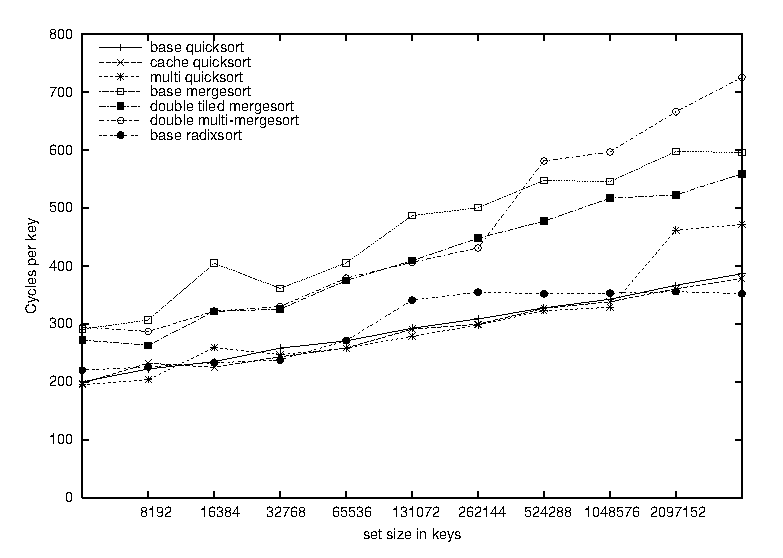
\includegraphics[angle=90,scale=1.8]{plots/all_cycles}
\vspace*{8em}
\end{changemargin}
\caption[Cycles per key of several major sorts and their variations]{\label{All
cycles}Cycles per key of several major sorts and their variations - this was
measured on a Pentium 4 using hardware performance counters.}
\end{figure}
\newpage
}

The best stable sort is memory-tuned radixsort. The best comparison-based stable
sort is double-aligned tiled mergesort. The best in-place sort is base
quicksort. The best in-place stable sort we examine in this report is insertion
sort. The best elementary sort is also insertion sort; as such it should be only
used for very small data sets. The best sort for very large data sets is
memory-tuned radixsort. The fastest overall sort was memory-tuned radixsort,
though all the base and memory-tuned quicksort are both very close.


\section{Contributions}


This section lists the contributions of this report. Each of these is novel  
and was discovered or developed during the course of this research.

The first main contribution of this report is that it repeats the work of LaMarca
on cache-conscious sorting, and validates many of his claims, while questioning
others. The other main contribution is having performed a branch prediction
analysis of major sorts - which to our knowledge has not been done before - and
developing a framework by which these results can be repeated and expanded upon.

Several discoveries were made and analysed: insertion sort has one misprediction
per key; selection sort has $O(H_N-1)$ branch mispredictions per key, which
applies to long arrays, though short arrays become more predictable the longer
they get, as in heapsort; tiling mergesort can be done in two steps, reducing
the cache miss count; aligning mergesort for a level 2 cache alone is
counter-productive - aligning it for level 1 and level 2 is significantly
faster; it is possible to avoid using a sentinel and still remove the bounds
check from a standard 2-heap, simply by reordering the steps involved;
sequential searches are far cheaper than binary searches across small lists, due
to a low branch misprediction rate. Bubblesort has terrible branch performance
in the middle, due to being partially sorted - it performs much worse than
selection sort as a result; multi-mergesort contains regular access patterns
which can be exploited by a two-level adaptive branch predictor; in almost all
other cases, two-level branch predictors are measurably less accurate than
simple bimodal predictors at predicting branches in sorting algorithms. A
median-of-three quicksort outperforms other medians; radixsort has no branch
mispredictions; shellsort has easily calculable branch mispredictions, and
performs very similarly to an $O(NlogN)$ sort. 

In addition, we provide an analysis of most major sorts currently used, a
comparison of $O(NlogN)$ sorts, of different medians for quicksort, of $O(N^2)$
sorts and of cache-conscious sorts. We present branch prediction performance
figures for most major sorts, and adapt cache-conscious strategies from
mergesort to not only significantly increase the performance of mergesort, but
also to make memory-tuned radixsort the fastest performing sort in our tests.

